%% LaTeX2e class for student theses
%% sections/content.tex
%%
%% Karlsruhe University of Applied Sciences
%% Faculty of  Computer Science and Business Information Systems
%% Distributed Systems (vsys)
%%
%% Prof. Dr. Christian Zirpins
%% christian.zirpins@hs-karlsruhe.de
%%
%%
%% Version 0.2, 2017-11-15
%%
%% --------------------------------------------------------
%% | Derived from sdqthesis by Erik Burger burger@kit.edu |
%% --------------------------------------------------------

\chapter{Entwurf einer Lösung für sichere Server-zu-Server Interaktion mit ActivityPub}
Zu Beginn dieses Kapitels ist die Frage zu stellen, wie die Architektur sicher gestaltet wird.

Eine Trennung der ActivityPub Komponenten in einen eigenen Service würde für eine isolierbare Ausführung sorgen. Es
\section{Entwurfsentscheidung}
Für die nachfolgende Architektur wurde sich in dieser Arbeit entschieden, da sie einen Modularen Charakter hat. Dies ist gegeben durch die Kapselung des Services in eine Express Middleware. Sowohl das alleinstehende betreiben des Services ist möglich als auch die Integration in einen bestehen Express Server.
\section{Technische Architektur}
	Der technischen Architektur liegt das Express Middleware Framework zugrunde. Der ActivityPub Service wird als Express Middleware, sowie als allein stehender Express Web Server implementiert. Bei der letzteren Variante wird anstatt die Middleware in ein bestehenden Express Server zu integrieren, ein eigener Express Server gestartet.\\
	\begin{figure}[h]
		\centering
		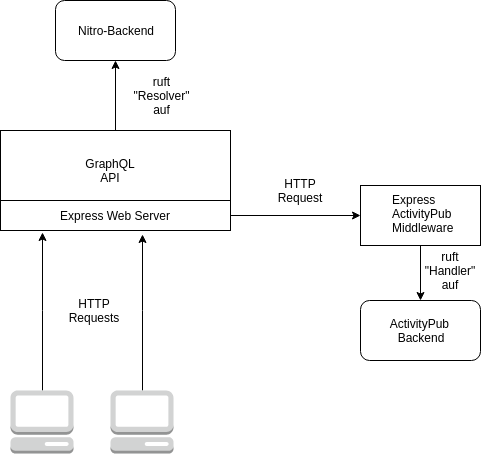
\includegraphics[scale=0.6]{figures/technische-architektur-activitypub.png}
		\label{technische-architektur-activitypub}
		\caption{Technische Architektur ActivityPub}
	\end{figure}
	In der oben gezeigten Abbildung wurde der ActivityPub Service in einen bestehenden Express Server einer GraphQL API integriert.\\
	
	Benutzer der API kommunizieren mit dem Web Server über das HTTP Protokoll. Der Web Server leitet die Anfragen dann an den entsprechenden Router weiter, welcher wiederum den Anfrage Inhalt transformiert und \glqq Handler\grqq~Funktionen des ActivityPub Service mit entsprechenden Parametern aufruft.\\
	
	\begin{figure}[h]
		\begin{minipage}{\textwidth}
			\centering
			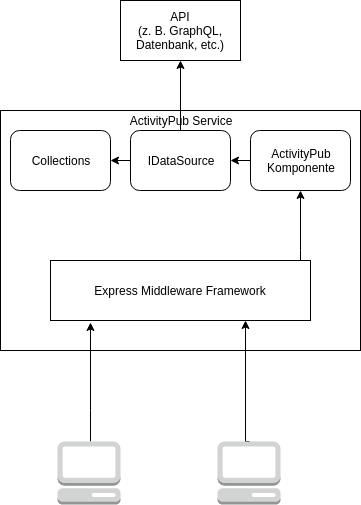
\includegraphics[scale=0.6]{figures/Technische-Architektur-standalone.png}
			\label{technische-architektur-standalone}
			\caption{Technische Architektur als allein stehender Server}
		\end{minipage}
	\end{figure}

	Die obige Abbildung zeigt eine detailliertere Variante des ActivityPub Service Diagramms aus Abb. 4.1.\\
	Es wird außerdem ersichtlich, dass, um eine maßgeschneiderte Version für ein weiteres Projekt zu erstellen, das Interface IDataSource implementiert werden muss.\\ 
	Sonst wird bei der Architektur weitestgehend darauf Wert gelegt, dass die meisten ActivityPub konformen Inhalte \glqq on the fly\grqq generiert werden können. Damit wird versucht für weitere Projekte die auf diesem Prototypen aufbauen wollen einen einfachen Einstieg zu bieten um andere Datenbanken o.ä. anbinden zu können.
